\documentclass{standalone}
\usepackage{tikz}
\begin{document}
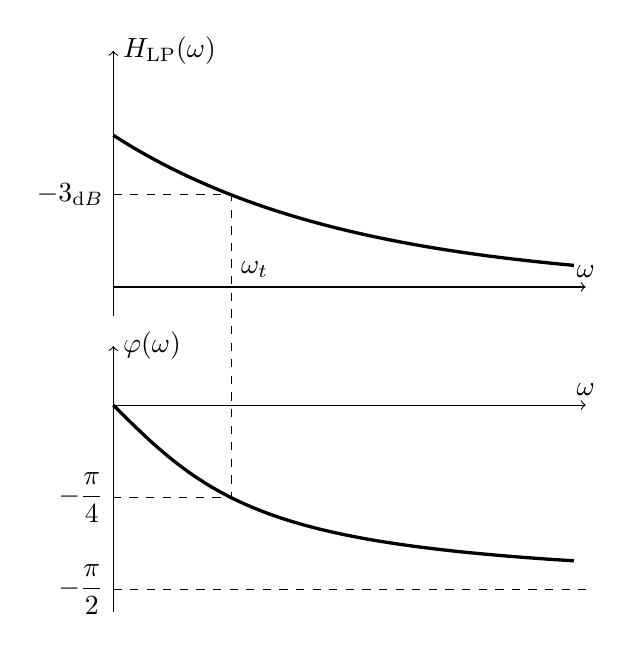
\begin{tikzpicture}[scale=1.5]
    \draw[->](0,1.75)--(0,4)node[right]{$H_{\mathrm{LP}}(\omega)$};
    \draw[->](0,2)--(4,2)node[above]{$\omega$};
    \draw[->](0,-0.75)--(0,1.5)node[right]{$\varphi(\omega)$};
    \draw[->](0,1)--(4,1)node[above]{$\omega$};
    \draw[very thick, smooth, domain=0:3.9]plot(\x,{2+e^(-0.5*(\x-0.5))});
    \draw[very thick, smooth, domain=0:3.9]plot(\x,{1+pi/180*atan(-\x)});
    \draw[dashed](0,2.779)node[left]{$-3_{\mathrm{d}B}$}--(1,2.779)--(1,2)node[above right]{$\omega_t$}--(1,0.215)--(0,0.215)node[left]{$-\displaystyle\frac{\pi}{4}$};
    \draw[dashed](0,-0.56)node[left]{$-\displaystyle\frac{\pi}{2}$}--(4,-0.56);
\end{tikzpicture}
\end{document}